% Chapter 3 -- translation by Doug Burkett & Tim Hutcheson (ca. 2001),
% lightly copy-edited for this edition.

\chapter{Direct current symbolic simulation}

\section{Definition of numerical simulation}

In the previous chapter we did several simulations, in which all of
the circuit element values were numerical. In addition, the
simulation results were also numerical. This type of simulation is
known as numerical simulation, and it is possible with any
conventional numeric simulator, such as Electronic Workbench, PSpice
and others. In these simulators it is possible to describe circuits
with dependent sources and find results for all nodes and elements,
but it is easier in Symbulator.

One reason that this task is easier in Symbulator, as compared to
the other simulators, is that Symbulator is a symbolic simulator,
not a numeric simulator. For example, dependent sources are treated
symbolically during the simulation, even though they may have
numerical values in the end. Another reason that Symbulator is
easier to use is that it was designed and developed by a student,
with the clear intent to provide other students with what they want
to receive as the answers of a simulation.

The full potential of Symbulator only becomes truly evident when we
run symbolic simulations.

\section{Definition of symbolic simulation}

A symbolic simulation is one in which at least one of the circuit
element values is not a number, be it real or complex, but instead a
symbolic value. This symbolic value may be an unknown variable, an
algebraic expression, a function of time or frequency, or some other
type of non-numerical expression.

We learned that the type of element entry will determine the type of
the results. The nature of the circuit element values is reflected
in the simulation answers. Exact values will produce exact answers.
Numerical values will produce numerical answers. So, symbolic values
will result in symbolic answers. We can be sure that a symbolic
simulation, having at least one symbolic value in the input circuit,
will have some symbolic answers.

\section{Symbolic simulation to obtain symbolic answers}

A simulation is considered symbolic if the circuit description
contains at least one element with a symbolic value. There are two
basic types of symbolic simulation: the first results in a symbolic
answer, and the second results in a numerical answer. The first type
of simulation, whose objective is a symbolic answer, is very useful
in design problems, and for getting expressions which symbolically
describe some circuit characteristic in terms of element values,
such as consumed power. It can also be used for academic purposes,
to demonstrate the laws of circuit analysis. Ohm's law, for example,
can be demonstrated by a Symbulator simulation. We shall try some
problems in order to learn to simulate symbolically.

\problem{012}

\emph{Problem: Demonstrate Ohm's law and the power dissipation
formula, with the following basic circuit and a symbolic
simulation.}


% figures added 10 Sep 2026
\begin{figure}[!ht]
\centering
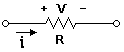
\includegraphics[width=42mm]{book_figures/p012_0.png}
\caption*{Circuit for Problem 012}
\end{figure}

Solution:

This is the simplest possible circuit. The first step is to name the
circuit nodes and elements. The second step is to run the simulation
with the circuit description:

\begin{entry}
sq\dc("r,1,0,r;j,0,1,i")
\end{entry}

Note the way in which the elements have been named: since there is
only one element of each type, we have used only one letter, which
is the first letter of the name of the element. We start the
simulation by pressing \key{ENTER}, then the status messages are
displayed, then `Done' is shown in the display. My calculator ran
this simulation in 6 seconds. Since this is the simplest possible
circuit, this is the shortest Symbulator simulation time. The
results are saved in the current folder.

We can demonstrate Ohm's law by displaying the value of \code{vr},
which is, as expected, \code{i*r} volts. To demonstrate the power
formula, we display the value of \code{pr}, which is
\code{i\^{}2*r} watts, which is correct.

We could also have verified Ohm's law by using a voltage source
instead of a current source, with this circuit description:

\begin{entry}
sq\dc("r,1,0,r;e,1,0,v")
\end{entry}

My calculator took 7 seconds to simulate this circuit. Note that a
voltage source takes more time than a current source. Although the
difference in this case is minor, only 1 second, the difference can
be considerable in more complicated circuits.

We demonstrate Ohm's law by displaying \code{ir}, which is
\code{v/r} amperes, which is another way to express the law. We
demonstrate the power formula by displaying \code{pr}, which is
\code{v\^{}2/r} watts and equivalent to the power expressed in terms
of the current.

This exercise teaches us that symbolic simulation is an easy way to
demonstrate and learn the basic laws of circuit analysis.

\section{Symbolic simulation to obtain numerical answers}

In some symbolic simulations, our objective is a numerical answer.
In this case, we use the \code{solve} command, the \code{solves}
tool and the (Expert) Mode.

Usually, to obtain a numerical answer, we need to know in advance
the numerical value of an answer---a voltage, current or power---for
each symbolic value in the input circuit.

\section{The solve command}

Let us see a simple example of the second type of symbolic
simulation, which obtains a numerical answer, using the \code{solve}
command.

\problem{013}

\emph{Problem: Determine the numerical values of $v_x$ and $i_x$ in
the following circuit.}


% figures added 10 Sep 2026
\begin{figure}[!ht]
\centering
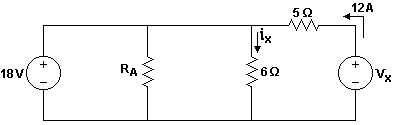
\includegraphics[width=134mm]{book_figures/p013_0.png}
\caption*{Circuit for Problem 013}
\end{figure}

% figures added 10 Sep 2026
\begin{figure}[!ht]
\centering
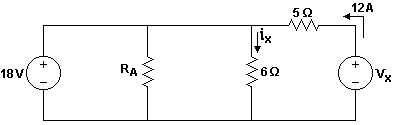
\includegraphics[width=134mm]{book_figures/p013_1.png}
\caption*{Circuit for Problem 013}
\end{figure}

Solution:

When we compare this circuit with previous examples, we see two
obvious differences. First, some element values are numeric and some
are symbolic. Second, we are given one of the branch currents: 12~A
through the 5 ohm resistor.

We first name the nodes and elements. We define the current
directions through the 5 and 6 ohm resistors as shown in the
drawing. For the symbolic values, we use the same names as shown in
the drawing. We must make sure that these variables do not already
exist in the current folder; that is, variable names \code{ra} and
\code{vx} must not exist, or the calculator will replace the
symbolic name with its stored value, and the simulation will be
incorrect. We use the \code{DelVar} command of the calculator to
delete the variables, like this:

\begin{entry}
DelVar ra,vx
\end{entry}

With this command, we tell the calculator: ``Delete the variables
\code{ra} and \code{vx} in the current folder''. There is no effect
if the variables do not actually exist. We could have deleted the
variables in the Var-Link window, but the method shown is faster.

Once the variables are deleted, we enter the circuit description and
run the simulation:

\begin{entry}
sq\dc("e1,1,0,18;ra,1,0,ra;r1,1,0,6;r2,2,1,5;ex,2,0,vx")
\end{entry}

We start the simulation by pressing \key{ENTER}, then the status
messages are shown, then `Done' is shown in the display. My
calculator took 16 seconds to simulate this circuit. The answers are
stored in the current folder.

We find $i_x$ by displaying the value of \code{ir1}, which is 3~A.
So far, there is nothing new about this problem.

The difference appears when we find $v_x$. First, it seems that we
could find $v_x$ by displaying the value of \code{v2}, but \code{v2}
is simply \code{vx} volts. Obviously, this answer does not tell us
anything new, because we require a numerical answer. Then, we
remember that the circuit drawing specifies that the current through
the 5 ohm resistor is 12~A. What is this current, according to the
Symbulator results? The recalled value of \code{ir2} is
\code{(vx-18)/5} amperes. This symbolic expression, the result of
the symbolic simulation, will help us find the value of $v_x$. How?
Let us see.

We know that the current is 12~A, and we have its expression as a
function of \code{vx}. We can combine these expressions in an
equation. When we solve the equation for the unknown \code{vx}, we
will find the numerical value of the voltage source. We could solve
this equation manually, but we will take advantage of the calculator
technology, and use the calculator's \code{solve} command. A
detailed explanation of this command can be found in the User's
Manual for the calculator. This is a very powerful command, which is
used extensively by Symbulator in its internal calculations. Now, we
will use \code{solve} manually, by entering this in the entry line:

\begin{entry}
solve(ir2=12,vx)
\end{entry}

With this command, we tell the calculator: ``Solve the equation
\code{ir2}~$= 12$ for the unknown \code{vx} and tell me the
answer''. In other words, what is the value of \code{vx} if
\code{ir2} is 12? We press \key{ENTER}, and almost instantly we
obtain the result: \code{vx}~$= 78$~volts. That easy! The unknown we
solved is the answer we wanted.

Having finished this problem, consider these three observations.

The \code{solve} command told us that \code{vx}~$= 78$, but it does
not store the value 78 in the variable \code{vx}. The \code{solve}
command solves equations for unknowns, and shows the results in the
display, but it does not store these results in the unknown
variables. To verify this, recall the value of \code{vx}, and
\code{vx} is shown. This means that no value is stored in variable
\code{vx}.

In this problem, the symbolic unknown in the circuit was also one of
the results the problem required. In other problems, this may not be
the case. We will see an example of this situation next.

The value of \code{ra} is indefinite. There is no mathematical way
we can obtain a numerical value for it. The reason is simple: to
obtain a numerical value for a symbolic element, we must know the
numerical value of an answer which involves the symbolic value, such
as a current, voltage or power. For example, we could find the value
of \code{vx} because we knew the numeric value of a current which is
a function of it. But we cannot find the value of \code{ra}, because
we are missing that clue: we do not know the numeric value of any
current, voltage or power that involves it.

I recommend that you review this problem until you feel you fully
understand the concepts it illustrates. Only then should you
continue.

\section{The solves tool}

The \code{solves} tool is part of the Symbulator. It is programmed
using technology developed for the Symbulator, and it has two
purposes: 1) to solve equations using the built-in \code{solve}
command, and 2) to store all the results in the appropriate
variables. This tool is executed with no input arguments between the
parentheses:

\begin{entry}
sq\solves()
\end{entry}

When we press \key{ENTER}, a dialog box is shown with two fields and
two options. The first field is for entering the equation or
equations we want to solve. The second field is for entering the
unknowns for which we want to solve. The two following options are
for choosing whether the solutions are real or complex, and whether
we want to use conditional equations, that is, known values. Press
\key{ESC} to return to the home screen.

Next we will solve a problem, similar to the previous one, which
shows the basic use of the \code{solves} tool.

\problem{014}

\emph{Problem: Determine the numerical values of $v_x$ and $i_x$ in
the following circuit.}


% figures added 10 Sep 2026
\begin{figure}[!ht]
\centering
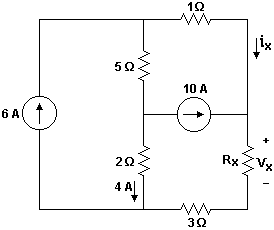
\includegraphics[width=93mm]{book_figures/p014_0.png}
\caption*{Circuit for Problem 014}
\end{figure}

% figures added 10 Sep 2026
\begin{figure}[!ht]
\centering
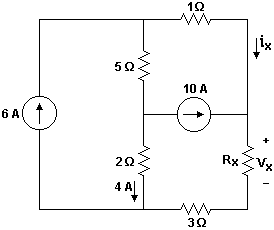
\includegraphics[width=93mm]{book_figures/p014_1.png}
\caption*{Circuit for Problem 014}
\end{figure}

Solution:

Note that in this circuit, the symbolic unknown is \code{rx}, while
the required answers are $i_x$ and $v_x$. These will likely be
functions of the unknown. For that reason, the strategy we must
follow is to simulate the circuit, solve for the unknown value of
the element, then obtain numerical values for the required answers.

First we name the nodes and elements. We define the currents through
the 1 and 2 ohm resistors as shown in the drawing. For the value of
the symbolic element, we use the same variable name as in the
drawing. To ensure that a variable of the same name does not already
exist, we use:

\begin{entry}
DelVar rx
\end{entry}

For the reference node, we use the lower left corner. The circuit
description and simulation command is:

\begin{entry}
sq\dc("j1,0,1,6;r1,1,2,1;r2,1,3,5;j2,3,2,10;r3,3,0,2;
      rx,2,4,rx;r4,4,0,3")
\end{entry}

We start the simulation with \key{ENTER}. `Done' is displayed after
the status messages are shown. My calculator took 30 seconds to run
this simulation. By this time, you have noticed that the simulation
time is proportional to the number of circuit nodes. The reason for
this is that Symbulator ``thinks nodally'', and will create an
equation for each circuit node except the reference. So, this
circuit with four nodes other than the reference takes approximately
four times as long as a circuit with one node other than the
reference. Obviously, there are other factors that affect the
simulation time, such as the type of analysis, the presence of
voltage sources and special elements, and symbolic values.

Returning to the problem, the simulation results are stored in the
current folder. We find $i_x$ by asking for the value of \code{ir1}.
We do not get a numerical value, but instead a function of
\code{rx}. The same happens for $v_x$: when we ask for \code{vrx},
we obtain a function of \code{rx}. As we expected, the numerical
answers we need are now functions of the unknown. In order to find
numerical values for $i_x$ and $v_x$, we must first find the
numerical value of \code{rx}. To allow us to find this value, the
problem has told us in advance that the current through the 2 ohm
resistor (which we have called \code{r3}) is 4~A.

The \code{solve} command is not the most appropriate for this task.
While we have seen that \code{solve} is extremely fast and effective
in solving equations, and could no doubt solve this small equation
in a thousandth of a second, \code{solve} would only display the
value of \code{rx} in the history screen, and not store the
numerical value. For that reason, \code{solves} is the more
appropriate tool.

To illustrate this point, first we will do the procedure with the
\code{solve} command. The first step is to solve the equation:

\begin{entry}
solve(ir3=4,rx)
\end{entry}

We obtain the answer \code{rx}~$= 40$. Since we will evaluate other
expressions which are functions of this unknown, we must manually
store this answer in the unknown variable, using the calculator
\code{Define} command, like this:

\begin{entry}
Define rx = 40
\end{entry}

Or, we could use the \key{STO} key, which is equivalent to
\code{Define}:

\begin{entry}
40 [STO] rx
\end{entry}

Once the value of \code{rx} is stored, we can ask the calculator for
the numerical values of $i_x$ and $v_x$. For \code{ir1} we obtain
$-8$~A, and for \code{vrx} we obtain 80~V.

We get the answers with this method, but it takes four steps: 1)
simulate the circuit, 2) solve for the unknown, 3) store the
unknown, and 4) evaluate the functions of the unknown.

With the \code{solves} tool, we find the answers in three steps: 1)
simulate the circuit, 2) solve and store the unknown in a single
step, and 3) evaluate the functions of the unknown to find the
answers. To demonstrate this, we first delete the variable
\code{rx}:

\begin{entry}
DelVar rx
\end{entry}

The simulation results are still stored in memory, so we will not
simulate the circuit again. Execute the \code{solves} tool:

\begin{entry}
sq\solves()
\end{entry}

The dialog box is shown. In the first field, labeled ``Equations'',
we enter the equation:

\begin{entry}
ir3=4
\end{entry}

In the second field, labeled ``Unknowns'', we enter the unknown:

\begin{entry}
rx
\end{entry}

Since the remaining options are real solutions and no conditionals,
we leave them unchanged. We press \key{ENTER}, twice if necessary. A
text message is shown to indicate that the tool is solving the
equations and then storing the answers. Next, the answer is shown:
\code{rx}~$= 40$. That is all. We press \key{ENTER} to return to the
home screen. The value 40 is now stored in the variable \code{rx}.
If you want to verify this, recall the value of \code{rx}, and 40 is
displayed.

The third step is to simply evaluate the required problem answers,
which are the numerical values of $i_x$ and $v_x$. For \code{ir1} we
obtain $-8$~A, and for \code{vrx} we obtain 80~V.

There is an even faster way to find these results, using the
(Expert) Mode. Since this method requires much more knowledge and
skill, we will dedicate the following chapter to it. Next we will
see another problem, similar to the last, to strengthen the concepts
we have learned.

\problem{015}

\emph{Problem: Determine the numerical values of $v_x$ and $i_x$ in
the following circuit.}


% figures added 10 Sep 2026
\begin{figure}[!ht]
\centering
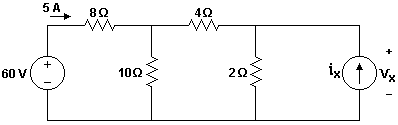
\includegraphics[width=135mm]{book_figures/p015_0.png}
\caption*{Circuit for Problem 015}
\end{figure}

% figures added 10 Sep 2026
\begin{figure}[!ht]
\centering
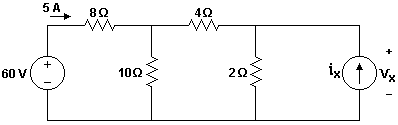
\includegraphics[width=135mm]{book_figures/p015_1.png}
\caption*{Circuit for Problem 015}
\end{figure}

Solution:

Note that the unknown symbolic current \code{ix} in this circuit is
also one of the required answers. The other required answer is
$v_x$, which will be a function of \code{ix}. We will simulate the
circuit, solve for the unknown, and then get the answers as
numerical values.

We name the nodes and elements, then define the direction of the
current through the 8 ohm resistor as shown in the drawing. We also
delete variable \code{ix}:

\begin{entry}
DelVar ix
\end{entry}

Using the bottom node as the reference node, we enter the circuit
description and run the simulation:

\begin{entry}
sq\dc("e1,1,0,60;r1,1,2,8;r2,2,0,10;r3,2,3,4;r4,3,0,2;jx,0,3,ix")
\end{entry}

We start the simulation by pressing \key{ENTER}. After the status
messages are shown, the display shows `Done'. My calculator took 19
seconds to run the simulation. All the symbolic results are in the
current folder. Since we know that the answers are symbolic, we must
solve for the unknown \code{ix}. Since one of the answers is a
function of \code{ix}, the best method is to use the \code{solves}
tool:

\begin{entry}
sq\solves()
\end{entry}

The input form is shown. If we have not deleted the variables in the
current folder after the last time we used \code{solves}, some
previous entries are shown in the input form. In the ``Equations''
field we enter the new equation, which replaces any previous
equation:

\begin{entry}
ir1=5
\end{entry}

In the second field, ``Unknowns'', we enter the unknown:

\begin{entry}
ix
\end{entry}

We leave the remaining options unchanged, since they are as we want
them. We press \key{ENTER}, twice if necessary. The answer
\code{ix}~$= 1$ is shown. We press \key{ENTER} to return to the home
screen, then we evaluate the remaining unknown: for \code{v3} we get
8 volts. Let us see yet another example of symbolic simulation with
numerical results.

\problem{016}

\emph{Problem: Find the value of $k$ such that voltage $v_y$ is
zero.}


% figures added 10 Sep 2026
\begin{figure}[!ht]
\centering
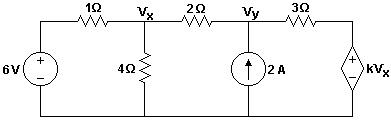
\includegraphics[width=133mm]{book_figures/p016_0.png}
\caption*{Circuit for Problem 016}
\end{figure}

% figures added 10 Sep 2026
\begin{figure}[!ht]
\centering
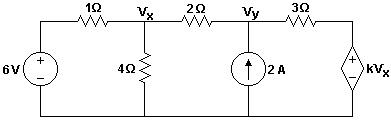
\includegraphics[width=133mm]{book_figures/p016_1.png}
\caption*{Circuit for Problem 016}
\end{figure}

Solution:

We label the nodes and elements. We label the center nodes \code{x}
and \code{y}, for obvious reasons. Delete variable \code{k}:

\begin{entry}
DelVar k
\end{entry}

Using the bottom node as the reference, we enter the circuit
description and run the simulation:

\begin{entry}
sq\dc("e1,1,0,6;r1,1,x,1;r2,x,0,4;r3,x,y,2;j1,0,y,2;
      r4,y,2,3;e2,2,0,k*vx")
\end{entry}

We start the simulation by pressing \key{ENTER}. After the status
messages are shown, `Done' is shown. My calculator took 36 seconds
to run the simulation. All results are in the current folder. Since
the only unknown is also the required answer, we can use the
built-in \code{solve} command:

\begin{entry}
solve(vy=0,k)
\end{entry}

We obtain the answer $k = -13/4$, which is correct. But how can we
be sure of this, for example, in the middle of a semester
examination?

\section{Verifying a symbolic simulation with a numerical answer}

There is an easy way to verify that the numerical answers to a
symbolic simulation are correct. All we need to do is get the
circuit description from the history area, instead of writing it
again, and replace all the symbolic values with the numeric values
that were found. To get the description from the history area, use
the same method described to correct errors, shown at the end of the
previous chapter.

After executing the simulation with numeric values, we evaluate the
previously known results, such as the voltages and currents. If we
get the same values that we knew before, then the symbolic
simulation results are correct.

As an example, we can verify the value for $k$ in the previous
problem with this numerical simulation:

\begin{entry}
sq\dc("e1,1,0,6;r1,1,x,1;r2,x,0,4;r3,x,y,2;j1,0,y,2;
      r4,y,2,3;e2,2,0,-13/4*vx")
\end{entry}

Notice that only the value of source \code{e2} has changed, which
now has a numeric value instead of the symbolic value \code{k}.
Recall that we were asked to find $k$ such that $v_y$ is zero.
Therefore, if the value found for $k$, $-13/4$, is correct, then the
voltage at node \code{y} should be zero. Ask for \code{vy} and you
will find it is 0~V. The answer has been verified.

Being able to verify answers is of special importance for a student
during an important examination. Many users recognize that
Symbulator is an excellent tool to verify answers during
examinations. This is probably one of its most significant
strengths.

Now we will learn to simulate like experts with Symbulator.
